\section{Procesamiento paralelo}\label{sec:paralel}

\subsection{Organizaciones con varios procesadores}

\subsubsection*{Tipos de sistemas paralelos}

La taxonomía introducida por Flynn es todavía la forma más común de clasificar a los sistemas según sus capacidades de procesamiento paralelo. Flynn propuso las siguientes categorías o clases de computadoras:

\begin{itemize}
  \item \textbf{Single Instruction Single Data (SISD):} un único procesador interpreta una única secuencia de instrucciones para operar con los datos almacenados en una única memoria. Los computadores monoprocesador caen dentro de esta categoría.
  \item \textbf{Single Instruction Multiple Data (SIMD):} una única máquina controla paso a paso la ejecución simultánea y sincronizada de un cierto número de elementos de proceso. Cada elemento de proceso tiene una memoria asociada, de forma que cada instrucción es ejecutada por cada procesador con un conjunto de datos diferentes. Los procesadores vectoriales y los matriciales pertenecen a esta categoría.
  \item \textbf{Multiple Instruction Single Data (MISD):} se transmite una secuencia de datos a un conjunto de procesadores, cada uno de los cuales ejecuta una secuencia de instrucciones diferente. Esta estructura nunca ha sido implementada.
  \item \textbf{Multiple Instruction Multiple Data (MIMD):} un conjunto de procesadores ejecuta simultáneamente secuencias de instrucciones diferentes con conjuntos de datos diferentes. Los SMP, los \textit{clusters} y los sistemas NUMA son ejemplos de esta categoría.
\end{itemize}

En la organización MIMD los procesadores son de uso general; cada uno es capaz de procesar todas las instrucciones necesarias para realizar las transformaciones apropiadas de los datos. Los computadores MIMD se pueden subdividir además según la forma que tienen los procesadores para comunicarse. Si los procesadores comparten una memoria común, entonces cada procesador accede a los programas y datos almacenados en la memoria compartida, y los procesadores se comunican unos con otros a través de esa memoria. La forma más común de este tipo de sistema se conoce como \textbf{multiprocesador simétrico (SMP)}. En un SMP, varios procesadores comparten una única memoria mediante un bus compartido u otro tipo de mecanismo de interconexión. Una característica distintiva de estos sistemas es que el tiempo de acceso a memoria principal es aproximadamente el mismo para cualquier procesador. Un desarrollo más reciente es la organización con \textbf{acceso no uniforme a memoria (NUMA)}. Como el propio nombre indica, el tiempo de acceso a zonas de memoria diferentes puede diferir en un computador NUMA.\@

Un conjunto de computadores monoprocesador independientes o de SMP pueden interconectarse para formar un \textit{cluster}. La comunicación entre los computadores se realiza mediante conexiones fijas o mediante algún tipo de red.

\begin{figure}[H]
  \centering
  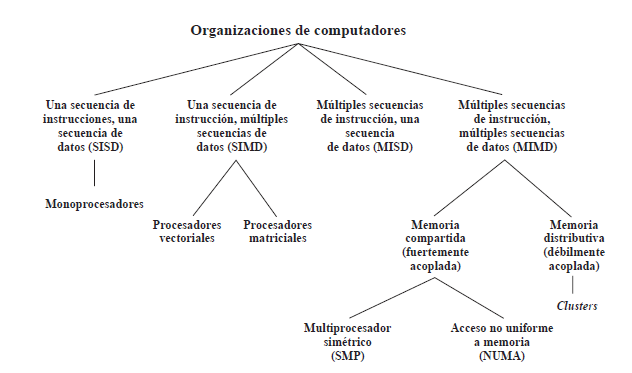
\includegraphics[width=0.7\textwidth]{Taxonomia.png}
  \caption{Taxonomía de las arquitecturas paralelas.}
\end{figure}

\subsection{Multiprocesadores simétricos}

\subsubsection{SMP}

El término SMP se refiere as la arquitectura hardware del computador y también al comportamiento del sistema operativo que utiliza dicha arquitectura. Un SMP puede definirse como un computador con las siguientes características:

\begin{itemize}
  \item Hay dos o más procesadores similares de capacidades comparables.
  \item Estos procesadores comparten la memoria principal y las E/S y están interconectados mediante un bus u otro tipo de sistema de interconexión, de forma que el tiempo de acceso a memoria es aproximadamente el mismo para todos los procesadores.
  \item Todos los procesadores comparten los dispositivos de E/S, bien a través de los mismos canales o mediante canales distintos que proporcionan caminos de acceso al mismo dispositivo.
  \item Todos los procesadores pueden desempeñar las mismas funciones.
  \item El sistema está controlado por un sistema operativo integrado que proporciona la interacción entre los procesadores y sus programas a los niveles de trabajo, tarea, fichero y datos.
\end{itemize}

El sistema operativo de un SMP planifica la distribución de procesos o hilos (\textit{threads}) entre todos los procesadores. Un SMP tiene las siguientes ventajas potenciales con respecto a una arquitectura monoprocesador:

\begin{itemize}
  \item \textbf{Prestaciones:} si el trabajo a realizar por un computador puede organizarse de forma que partes del mismo se puedan realizar en paralelo, entonces un sistema con varios procesadores proporcionará mejores prestaciones que uno con un solo procesador del mismo tipo.
  \item \textbf{Disponibilidad:} en un multiprocesador simétrico, debido a que todos los procesadores pueden realizar las mismas funciones, un fallo en un procesador no hará que el computador se detenga.
  \item \textbf{Crecimiento incremental:} se pueden aumentar las prestaciones del sistema añadiendo más procesadores.
  \item \textbf{Escalado:} los fabricantes pueden ofrecer una gama de productos con precios y prestaciones diferentes en función del número de procesadores que configuran el sistema.
\end{itemize}

Una característica atractiva de un SMP es que la existencia de varios procesadores es transparente al usuario. El sistema operativo se encarga de la sincronización entre los procesadores y de la planificación de los hilos o de los procesos, asignándolos a los distintos procesadores.

\subsubsection*{Bus de tiempo compartido}

La organización más común en los computadores personales, estaciones de trabajo y servidores es el bus de tiempo compartido. El bus de tiempo compartido es el mecanismo más simple para construir un sistema multiprocesador. La estructura y las interfaces son básicamente las mismas que las de un sistema de un único procesador que utilice un bus para la interconexión. El bus consta de líneas de control, dirección y datos. Para facilitar las transferencias de DMA con los procesadores de E/S, se proporcionan los elementos para el:

\begin{itemize}
  \item \textbf{Direccionamiento:} debe ser posible distinguir los módulos del bus para determinar la fuente y el destino de los datos.
  \item \textbf{Arbitraje:} cualquier módulo de E/S puede funcionar temporalmente como un \textit{maestro}. Se proporciona un mecanismo para arbitrar entre las peticiones que compiten por el control del bus, utilizando algún tiempo de esquema de prioridad.
  \item \textbf{Tiempo compartido:} cuando un módulo está controlando el bus, los otros módulos no tienen acceso al mismo y deben, si es necesario, suspender su operación hasta que dispongan del bus.
\end{itemize}

La organización del bus presenta varias características atractivas:

\begin{itemize}
  \item \textbf{Simplicidad:} es la aproximación más simple para organizar el multiprocesador. La interfaz física y la lógica de cada procesador para el direccionamiento, el arbitraje y para compartir el tiempo del bus es el mismo que de un sistema con un solo procesador.
  \item \textbf{Flexibilidad:} es generalmente sencillo de expandir el sistema conectando más procesadores al bus.
  \item \textbf{Fiabilidad:} el bus es esencialmente un medio pasivo, y el fallo de cualquiera de los dispositivos conectados no provocaría el fallo de todo el sistema.
\end{itemize}

La principal desventaja de la organización de bus son las prestaciones. Todas las referencias a memoria pasan por el bus. En consecuencia, la velocidad del sistema está limitada por el tiempo de ciclo. Para mejorar las prestaciones, es deseable equipar a cada procesador con una memoria caché.

El uso de cachés introduce algunas consideraciones de diseño nuevas. Puesto que cada caché local contiene una imagen de una parte de la memoria, si se altera una palabra en una caché, es concebible que eso podría invalidar una palabra en otra caché. Para evitarlo, se debe avisar a los otros procesadores de que se ha producido una actualización de memoria. Este problema se conoce como \textit{coherencia de caché}.

\subsubsection{Clusters}

Los \textbf{clusters} constituyen la alternativa a los multiprocesadores simétricos (SMP) para disponer de prestaciones y disponibilidad elevadas, y son particularmente atractivos en aplicaciones propias de un servidor. Se puede definir un \textbf{cluster} como un grupo de computadores completos interconectados que trabajan conjuntamente como un único recurso de cómputo, creándose la ilusión de que se trata de una sola maquina.

Los objetivos de los clusters son:

\begin{itemize}
  \item \textbf{Escalabilidad absoluta:} es posible configurar clusters grande que incluso superan las prestaciones de los computadores independientes más potentes. Un cluster puede tener decenas de máquinas, cada una de las cuales puede ser un multiprocesador.
  \item \textbf{Escalabilidad incremental:} un cluster se configura de forma que sea posible añadir nuevos sistemas al cluster en ampliaciones sucesivas.
  \item \textbf{Alta disponibilidad:} puesto que cada nodo del cluster es un computador autónomo, el fallo de uno de los nodo no significa la perdida del servicio.
  \item \textbf{Mejor relación precio-prestaciones:} al utilizar elementos estandarizados, es posible configurar un cluster con mayor o igual potencia de cómputo que un ordenador independiente mayor, a mucho menos costo.
\end{itemize}

\subsubsection*{Arquitectura de los clusters}

Los computadores se conectan a través de una red de área loca de alta velocidad o mediante un conmutador. Cada computador puede trabajar de forma independiente. Además, en cada computador se instala una capa software intermedia que permite el funcionamiento de todos los computadores como un único cluster. El \textit{middleware del cluster} proporciona al usuario una imagen unificada conocida como \textbf{imagen de sistema único}. El \textit{middleware} también es responsable de proporcionar alta disponibilidad, distribuyendo la carga y respondiendo a los fallos de los componentes. Se pueden enumerar los siguientes servicios y funciones deseables en la capa de middleware:

\begin{itemize}
  \item Punto de entrada único.
  \item Jerarquía de ficheros única.
  \item Punto de control único.
  \item Red virtual única.
  \item Espacio de memoria único.
  \item Sistema de gestión de trabajos único.
  \item Interfaz de usuario única.
  \item Espacio de E/S único.
  \item Espacio de procesos único.
  \item Puntos de chequeo.
  \item Migración de procesos.
\end{itemize}

\begin{figure}[H]
  \centering
  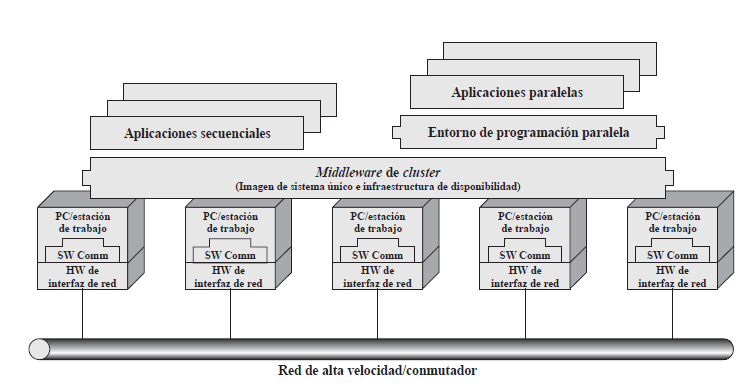
\includegraphics[width=0.7\textwidth]{Cluster.png}
  \caption{Arquitectura de computador de cluster}
\end{figure}

\subsubsection*{Clusters frente a sistemas SMP}

La principal ventaja de un SMP es que resulta más fácil gestionar y configurar que un cluster. El SMP está mucho más cerca del modelo de computador de un solo procesador para el que están disponibles casi todas las aplicaciones. El principal cambio que se necesita para pasar de un computador monoprocesador a un SMP se refiere al funcionamiento del planificador. Otra ventaja es que los SMP ocupan menos espacio físico y y consume menos energía.

Con el tiempo los clusters dominarán el mercado de servidores de altas prestaciones. Los cluster son superiores a los SMP en términos de escalabilidad absoluta e incremental, y además también son superiores en términos de disponibilidad.

\subsection{Coherencia de caché}

En los sistemas multiprocesador contemporáneos es común disponer de uno o dos niveles de caché asociados a cada procesador. Esta organización es esencial para conseguir unas prestaciones razonables. No obstante, origina un problema conocido como \textbf{coherencia de caché}. La esencia del problema es esta: pueden existir varias copias del mismo dato simultáneamente en cachés diferentes, y si los procesadores actualizan sus copias, puede producirse una visión inconsistente de la memoria.

El objetivo de un protocolo de coherencia de caché, es situar las variables locales utilizadas recientemente en la caché apropiada y mantenerlas allí para las distintas escrituras y lecturas, al mismo tiempo que se mantiene la consistencia de las variables compartidas que pudieran encontrarse en varias cachés al mismo tiempo.

\subsubsection{Protocolos de directorio}

 Los protocolos de directorio son utilizados para recopilar y mantener información sobre la ubicación de las copias de líneas en un sistema. Hay un controlador centralizado y un directorio almacenado en la memoria principal. El controlador centralizado verifica y emite instrucciones para transferir datos entre la memoria y las cachés. También se encarga de mantener actualizada la información de estado. Antes de que un procesador pueda escribir en una copia local de una línea, debe solicitar acceso exclusivo al controlador. Este controlador envía un mensaje a los procesadores con copias de la línea, obligándolos a invalidar sus copias. Después de recibir confirmación de los procesadores, se concede acceso exclusivo al procesador solicitante. Si otro procesador intenta leer una línea en acceso exclusivo, se envía una notificación al controlador, quien ordena al procesador poseedor de la línea volver a escribirla en memoria principal. Aunque los esquemas de directorio tienen desventajas como un cuello de botella central y un costo de comunicación elevado, son efectivos en sistemas de gran escala con múltiples buses o complejas interconexiones.

 \subsubsection{Protocolos de sondeo}

 Los protocolos de sondeo distribuyen la responsabilidad de mantener la coherencia de caché entre los controladores de caché en un sistema multiprocesador. Estos protocolos se adaptan bien a sistemas basados en un bus compartido, ya que el bus proporciona una forma sencilla de difusión y sondeo.

Existen dos enfoques principales en los protocolos de sondeo: \textit{invalidar-si-escritura} y \textit{actualizar-si-escritura} o \textit{difundir-escritura}. En el enfoque de \textit{invalidar-si-escritura}, cuando una caché realiza una escritura en una línea compartida, envía una notificación que invalida la línea en las otras cachés, asegurando que la línea sea exclusiva para la caché que realizó la escritura. En el enfoque de \textit{actualizar-si-escritura}, cuando una caché desea escribir en una línea compartida, la palabra actualizada se distribuye a las demás cachés que contienen esa línea, permitiendo que todas las cachés la actualicen.

No hay un enfoque que sea mejor en todas las situaciones, ya que las prestaciones dependen del número de cachés locales y del patrón de escrituras y lecturas en la memoria. Es importante tener en cuenta que aunque los protocolos de sondeo permiten mantener la coherencia de caché, también pueden aumentar el tráfico en el bus compartido, lo cual puede afectar los beneficios de las cachés locales.

En resumen, los protocolos de sondeo son utilizados para mantener la coherencia de caché en sistemas multiprocesador, distribuyendo la responsabilidad entre los controladores de caché. Hay dos enfoques principales: \textit{invalidar-si-escritura} y \textit{actualizar-si-escritura}. La elección del enfoque depende del número de cachés y del patrón de acceso a memoria. Es importante considerar el impacto en el tráfico del bus compartido al implementar estos protocolos.

\subsection{Acceso no uniforme a memoria}

\begin{itemize}
  \item \textbf{Uniform Memory Access (UMA):} todos los procesadores pueden acceder a toda la memoria principal utilizando instrucciones de carga y almacenamiento. El tiempo de acceso de un procesador a cualquier región de la memoria es el mismo.
  \item \textbf{Nonuniform Memory Access (NUMA):} todos los procesadores tiene acceso a todas las partes de la memoria principal utilizando instrucciones de carga y almacenamiento. El tiempo de acceso a memoria de un procesador depende de la región a la que se acceda.   
  \item \textbf{Cache-Coherent NUMA (CC-NUMA):} un computador NUMA en el que la coherencia de caché se mantiene en todas las cachés de los distintos procesadores.
\end{itemize}

\subsubsection*{Motivación}

En un SMP existe un límite práctico en el número de procesadores que pueden utilizarse. Un esquema de caché eficaz reduce el tráfico en el bus entre los procesadores y la memoria principal. La degradación de las prestaciones parece que limita el número de procesadores en una configuración SMP entre 16 y 64 procesadores.

Precisamente el límite de procesadores en un SMP es uno de los motivos para el desarrollo de los clusters. Sin embargo, en un cluster cada nodo tiene su propia memoria principal privada y las aplicaciones no ven la memoria global. La coherencia se mantiene mediante software en lugar de mediante hardware.

El objetivo de un computador NUMA es mantener una memoria transparente desde cualquier parte del sistema, al tiempo que se permiten varios nodos de multiprocesador, cada uno con su propio bus u otro sistema de interconexión interna.

\subsubsection*{Organización}

Cada nodo de un sistema CC-NUMA incluye cierta cantidad de memoria principal. Sin embargo, desde el punto de vista de los procesadores, existe un único espacio de memoria direccionable en el que a cada posición se asocia una única dirección válida para todo el sistema. Cuando un procesador inicia un acceso a memoria, si la posición solicitada no se encuentra en la caché del procesador, entonces la caché L2 inicia una operación de captación. Si la línea deseada está en una posición remota de la memoria principal, la línea se capta a través del bus local. Si la línea solicitada está en una porción remota de la memoria, entonces se envía una petición automática para captar dicha línea a través de la red de interconexión, se proporciona a través del bus local a la caché que lo solicitaba en dicho bus.

\begin{figure}[H]
  \centering
  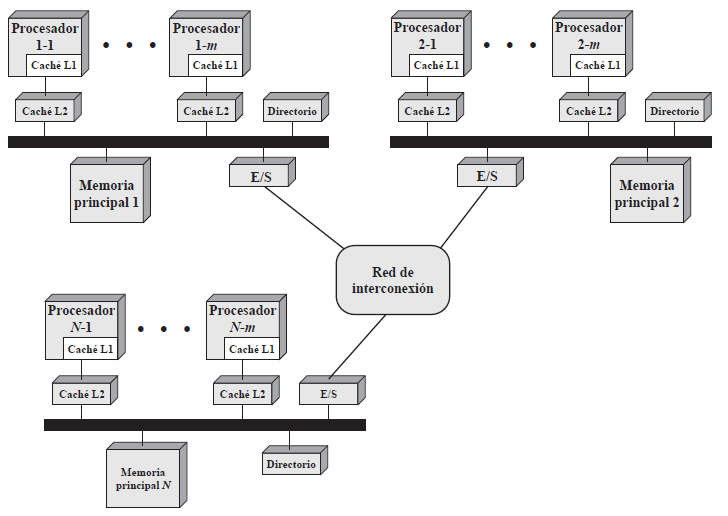
\includegraphics[width=0.7\textwidth]{OrganizacionCCNUMA.png}
  \caption{Organización CC-NUMA}
\end{figure}

\subsection{Procesamiento multihebra}

Una alternativa, que permite un paralelismo entre instrucciones elevado sin incrementar ni la complejidad de los circuitos ni el consumo de potencia, es el procesamiento multihebra. Básicamente, la secuencia de instrucciones se divide en secuencias más pequeñas, denominadas hebras.

\subsubsection{Procesamiento multihebra implicito y explícito}

El concepto de hebra utilizado para estudiar los procesadores multihebra puede no ser el mismo que el concepto de hebra en un sistema operativo multiprogramado. Por lo tanto, es útil definir brevemente una seria de termino:

\begin{itemize}
  \item \textbf{Proceso:} un programa en ejecución en un computador.
  \begin{itemize}
    \item \textit{Propiedad de recursos:} espacio de direcciones virtuales para almacenar la imagen de un proceso.
    \item \textit{Planificación/Ejecución:} hay un camino de ejecución (traza).
  \end{itemize}
  \item \textbf{Conmutación de proceso:} operación que cambia el proceso que se está ejecutando en el procesador por otro.
  \item \textbf{Hebra:} una unidad de trabajo dentro de un proceso que se puede asignar al procesador. Incluye un contexto de procesador (con el contador de programa y el puntero de pila) y su propia área de datos para la pila.
  \item \textbf{Conmutación de hebra:} el control del procesador pasa de una hebra a otra dentro de un mismo proceso.
\end{itemize}

\begin{itemize}
  \item \textbf{Multihebra explícito:} se realiza una ejecución concurrente de instrucciones de diferentes hebras explícitas. Se mezclan instrucciones de diferentes hebras en cauces compartidos o se ejecuta de manera paralela en cauces paralelos. Todos los procesadores comerciales lo usan.
  \item \textbf{Multihebra implícito:} se realiza una ejecución concurrente de varias hebras extraídas de un único programa secuencial. Se definen estáticamente por el compilador o dinámicamente por el hardware.
\end{itemize}

En un procesador multihebra el PC es distinto para cada hebra, permitiendo la ejecución concurrente. Cada hebra es tratada por separado, predicción de saltos, renombre de registros para optimizar ejecución.